\titledquestion{理解 word2vec}[15]
回想一下 {\tt word2vec} 背后的关键洞见是：\textit{“一个词是由它周围的词所定义的”}。具体来说，考虑一个“中心词”$c$，它前后都有一定长度的上下文。我们将这个上下文窗口中的词称为“外部词”($O$)。例如，在图~\ref{fig:word2vec} 中，上下文窗口长度为 2，中心词 $c$ 是 `banking`，外部词分别是 `turning`、`into`、`crises` 和 `as`：

\begin{figure}[h]
    \centering
    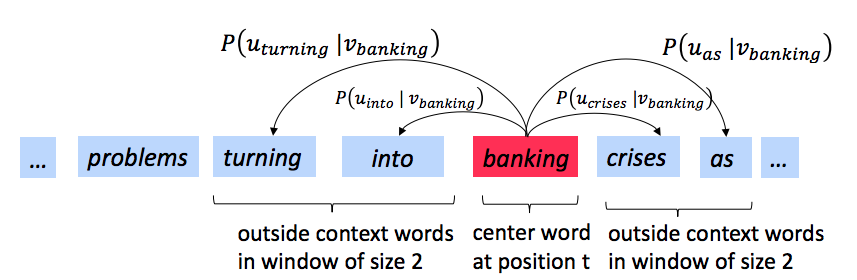
\includegraphics[width=0.6\textwidth]{word2vec.png}
    \caption{窗口大小为 2 的 word2vec skip-gram 预测模型}
    \label{fig:word2vec}
\end{figure}

Skip-gram {\tt word2vec} 旨在学习概率分布 $P(O|C)$。具体地说，给定一个特定词 $o$ 和一个特定词 $c$，我们想预测 $P(O=o|C=c)$：词 $o$ 是 $c$ 的“外部词”的概率（也就是说，它落在 $c$ 的上下文窗口中）。
我们通过对一系列向量点积取 softmax 来建模这个概率：% 我加了 “softmax” 这个词，因为我猜很多学生会忘记它是什么，以及为什么损失函数被称为 naive softmax；如果太啰嗦也可以删掉

\begin{equation}
 P(O=o \mid C=c) = \frac{\exp(\bu_{o}^\top \bv_c)}{\sum_{w \in \text{Vocab}} \exp(\bu_{w}^\top \bv_c)}
 \label{word2vec_condprob}
\end{equation}

对每个词，我们学习两个向量 $u$ 和 $v$，其中 $\bu_o$ 是表示外部词 $o$ 的“外部”向量，$\bv_c$ 是表示中心词 $c$ 的“中心”向量。
我们把这些参数存储在两个矩阵 $\bU$ 和 $\bV$ 中。
$\bU$ 的列是所有“外部”向量 $\bu_{w}$；
$\bV$ 的列是所有“中心”向量 $\bv_{w}$。
$\bU$ 和 $\bV$ 都为词表中的每个 $w \in \text{Vocabulary}$ 保存一个向量。\footnote{假设词表中的每个词都对应一个整数编号 $k$。粗体小写字母表示向量。$\bu_k$ 同时表示 $\bU$ 的第 $k$ 列，以及索引为 $k$ 的词对应的“外部词”向量。$\bv_k$ 同时表示 $\bV$ 的第 $k$ 列，以及索引为 $k$ 的词对应的“中心词”向量。\textbf{为了简化记号，我们将交替使用 $k$ 表示词 $k$ 以及词 $k$ 的索引。}}\newline

%我们可以把概率分布 $P(O|C)$ 视为一个可以通过监督学习逼近的预测函数。对于任意训练样本，我们都有一个 $o$ 和 $c$。我们随后会计算一个值 $P(O=o|C=c)$ 并记录损失。
回顾课堂内容，对于一对单词 $c$ 和 $o$，损失函数为：

\begin{equation} 
\bJ_{\text{naive-softmax}}(\bv_c, o, \bU) = -\log P(O=o| C=c).
\label{naive-softmax}
\end{equation}

我们可以把这个损失看成真实分布 $\by$ 与预测分布 $\hat{\by}$ 之间的交叉熵\footnote{真实（离散）概率分布 $p$ 与另一个分布 $q$ 之间的\textbf{交叉熵损失}是 $-\sum_i p_i \log(q_i)$。}，对应于特定中心词 $c$ 和特定外部词 $o$。
这里，$\by$ 和 $\hat{\by}$ 都是长度等于词表大小的向量。
进一步地，这些向量的第 $k$ 项表示给定中心词 $c$ 时，第 $k$ 个词成为“外部词”的条件概率。
真实经验分布 $\by$ 是一个 one-hot 向量：对于真实外部词 $o$，对应位置为 1，其余位置为 0，这对应于某个特定中心词 $c$ 和外部词 $o$ 的一个样本。\footnote{注意，整个训练数据的真实条件概率分布并不一定是 one-hot。}
预测分布 $\hat{\by}$ 是我们模型在式（\ref{word2vec_condprob}）中给出的概率分布 $P(O|C=c)$。\newline

\textbf{注意：} 在本作业中，计算导数时，请使用课堂中复习过的方法（即不要使用泰勒级数近似）。

\clearpage
\begin{parts}
\part[2]
证明 naive-softmax loss（式 \ref{naive-softmax}）与 $\by$ 和 $\hat{\by}$ 之间的交叉熵损失相同，也就是（注意 $\by$（真实分布）、$\hat{\by}$（预测分布）都是向量，$\hat{\by}_o$ 是标量）：

\begin{equation}
\by_w =
\begin{cases}
1, & w=o,\\
0, & w\neq o,
\end{cases}
\qquad\Rightarrow\qquad
-\sum_{w \in \text{Vocab}} \by_w \log(\hat{\by}_w)
= -\log(\hat{\by}_o).
\end{equation}

因为真实分布 $\by$ 是 one-hot 向量，只有真实外部词 $o$ 那一项为 1，其余为 0，所以交叉熵只保留第 $o$ 项；而 $\hat{\by}_o = P(O=o\mid C=c)$，因此
\[
J_{\text{naive-softmax}}(\bv_c,o,\bU)
= -\log P(O=o\mid C=c)
= -\log(\hat{\by}_o)
= -\sum_{w \in \text{Vocab}} \by_w \log(\hat{\by}_w).
\]


% Question 1-B
\part[6]
\begin{enumerate}[label=\roman*.]
    \item 
    计算 $\bJ_{\text{naive-softmax}}(\bv_c, o, \bU)$ 相对于 $\bv_c$ 的偏导数。\emph{请用 $\by$、$\hat{\by}$、$\bU$ 的形式写出答案，并展示你的推导过程以获得满分。}
    \begin{itemize} 
        \item \textbf{注意：} 最终偏导数的答案应遵循形状约定：任意函数 $f(x)$ 相对于 $x$ 的偏导数必须与 $x$ 具有\textbf{相同形状}。\footnote{这样可以让我们使用梯度下降高效最小化函数，而不必担心重塑或维度不匹配。在遵守形状约定的情况下，我们保证 $\theta:= \theta - \alpha\frac{\partial J(\theta)}{\partial \theta}$ 是一个良定义的更新规则。}
        \item 请以向量化形式给出偏导数答案。例如，当我们要求你用 $\by$、$\hat{\by}$ 和 $\bU$ 表达答案时，你在最终答案中不能引用这些项的特定元素（例如 $\by_1$、$\by_2$、$\dots$）。
    \end{itemize}
    \item
    当你计算出的梯度等于零时，什么情况下会发生？ \\
    \textbf{提示：} 你可能需要复习并使用一些基础线性代数概念。
    \item
    你找到的梯度是两个项之差。请解释这两个项分别如何在将梯度从词向量 $v_c$ 中减去时改善词向量。

\end{enumerate}



% Question 1-C
\part[1]
在许多使用词嵌入的下游应用中，通常使用 L2 归一化向量（例如 $\mathbf{u}/||\mathbf{u}||_2$，其中 $||\mathbf{u}||_2 = \sqrt{\sum_i u_i^2}$）而不是原始形式（例如 $\mathbf{u}$）。考虑一个假设的二分类下游任务：判断短语是正向还是负向，你根据单词嵌入的和来决定符号。在什么情况下，L2 归一化会丢失有用信息？在什么情况下不会？

\textbf{提示：} 考虑 $\mathbf{u}_x = \alpha\mathbf{u}_y$ 的情况，其中 $x \neq y$ 且 $\alpha$ 是某个标量。当 $\alpha$ 为正时，归一化后的 $\mathbf{u}_x$ 和 $\mathbf{u}_y$ 会是什么？如果这类归一化会影响或不会影响最终分类，$\mathbf{u}_x$ 和 $\mathbf{u}_y$ 可能具有什么关系？


% Question 1-D
\part[5] 
计算 $\bJ_{\text{naive-softmax}}(\bv_c, o, \bU)$ 相对于每个“外部词”向量 $\bu_w$ 的偏导数。分两种情况：当 $w=o$ 时，这是真实的“外部词”向量；当 $w \neq o$ 时，这是其他所有词的向量。请用 $\by$、$\hat{\by}$ 和 $\bv_c$ 表达答案。在这一小问中，你也可以引用这些项中的具体元素（例如 $\by_1$、$\by_2$、$\dots$）。注意，$\bu_w$ 是一个向量，而 $\by_1, \by_2, \dots$ 是标量。展示你的推导过程以获得满分。



% Question 1-E
\part[1]
写出 $\bJ_{\text{naive-softmax}}(\bv_c, o, \bU)$ 相对于 $\bU$ 的偏导数。请按列向量 $\frac{\partial \bJ(\bv_c, o, \bU)}{\partial \bu_1}$、$\frac{\partial \bJ(\bv_c, o, \bU)}{\partial \bu_2}$、$\cdots$、$\frac{\partial \bJ(\bv_c, o, \bU)}{\partial \bu_{|\text{Vocab}|}}$ 来分解答案。不需要推导，只需给出符合矩阵形式的答案。


\end{parts}